\documentclass[a4paper]{article}

%------------------------------------------------------------
\usepackage[a4paper, total={6in, 9in}]{geometry}
\usepackage{amsmath}
\usepackage{booktabs}
\usepackage{caption}
\usepackage{enumitem}
\usepackage{graphicx}
\usepackage{float}
\usepackage{inconsolata}
\usepackage{listings}
\usepackage{pstricks-add}
\usepackage{siunitx}
\usepackage[most]{tcolorbox}
\usepackage{tikz}
\usepackage{epstopdf} %converting to PDF
\usepackage{hyperref}

\usetikzlibrary{shapes.geometric}

%------------------------------------------------------------
\graphicspath{{./fig/}}

%------------------------------------------------------------
\setlength{\parindent}{0in}

\lstdefinestyle{Python}{
	language        = Python,
	basicstyle      = \ttfamily,
	keywordstyle    = \color{blue},
	keywordstyle    = [2] \color{teal}, % just to check that it works
	stringstyle     = \color{green},
	commentstyle    = \color{red}\ttfamily
}

%------------------------------------------------------------
\newtcblisting[auto counter]{sexylisting}[2][]{sharp corners, 
    fonttitle=\bfseries, colframe=gray, listing only, 
    listing options={basicstyle=\ttfamily,language=Python}, 
    title=Listing \thetcbcounter: #2, #1}

%------------------------------------------------------------
\tikzstyle{block} = [draw, fill=blue!20, rectangle, 
    minimum height=3em, minimum width=3em]
\tikzstyle{sum} = [draw, fill=blue!20, circle, node distance=1cm]
\tikzstyle{input} = [coordinate]
\tikzstyle{output} = [coordinate]
\tikzstyle{pinstyle} = [pin edge={to-,thin,black}]

%------------------------------------------------------------

\begin{document}
\title{Localisation: Where Am I?}
\author{Shane Reynolds}
\maketitle
\tableofcontents
\newpage
\section{Introduction}
Suppose a robot has an unknown pose in an environment for which it has a map. The robot takes sensor readings, and based on these observations, must infer a set of poses where it could be located in the environment. In robotics, this scenario is known as the \textit{localisation problem} \cite{Cox:1991, Wang:1988}. In simpler terms, localisation is the problem of estimating a mobile robot's location and orientation relative to its environment, given sensor data \cite{Thrun:2001}. This is not as straight forward as it appears given robot actuators can only are subject to small random perturbations in performance, and sensors provide imperfect measurement. Compounding these problems is the fact that the robot may not even know it's initial pose relative to the environment. This paper explores two approaches to solving the localisation problem, after providing a brief discussion on the common variations of the problem. The first of these solutions is the Extended Kalman Filter (EKF): an adaptation of the Kalman Filter, suited to the estimation of non-linear system responses. The second solution is a particle filter method called Monte Carlo Localisation (MCL). The paper concludes with an application of MCL in a Gazebo simulation using an off-the-shelf MCL package in ROS. The MCL implementation is trialled across two different robot models providing opportunities for discussion of implementation robustness, and an analysis of parameter tuning for reliable performance.

\section{Background}
The mobile robot localisation problem comes in three flavours. The simplest involves tracking the robot's pose relative to its environment - called \textit{position tracking}. This scenario requires an initial known estimate of the robot's pose relative to the environment. Robot actions require pose updates using noisey sensor data \cite{Thrun:1999}. Often initial pose estimates are unavailable - this scenario represents a more meaningful problem version called the \textit{global localisation problem}. The goal here is for the robot determine it's pose from scratch, given it is unaware of the initial pose. Finally, the most challenging problem type is referred to as the \textit{kidnapped robot problem} which sees a localised robot tele-ported to another location on the map without knowledge of the move. This is different to the \textit{global localisation problem} scenario because, after tele-porting, the robot incorrectly believes it is somewhere other than its current location. This final scenario is used to test whether a localisation algorithm can recover from a catastrophic failure.

\subsection{Kalman Filters}
Kalman Filters can be used to solve the simplest localisation problem: position tracking. In an ideal world, position tracking is a trivial task in which the robot knows it's starting location, and updates position with perfect actuation and perfect sensor readings. In the real world, however, this is not the case. Actuation is not perfect, and is subject to minor perturbations, or wheel slippage can occur. Furthermore, sensor readings are noisey. The implications are that both movement and measurement are imprecise and subject to stochastic errors. Consider the a mobile robot moving along a one dimensional trajectory. Let the discrete time position be $x_j$, at time $j$. We note that the position at time $j$ is dependent on the previous position at time $j-1$, denoted as $x_{j-1}$, plus any movement action taken by the robot, denoted as $u_j$. Additionally, as previously noted, the robot's actuators are not perfect and are subject to noise, $\omega_j$. We can write $x_j$ as follows:
\begin{equation}
x_j = a \cdot x_j + b \cdot u_j + \omega_j
\end{equation}

This description is sometimes easier to understand when visualised as a computational block diagram, shown in Figure 1.
\begin{figure}[h]
\centering
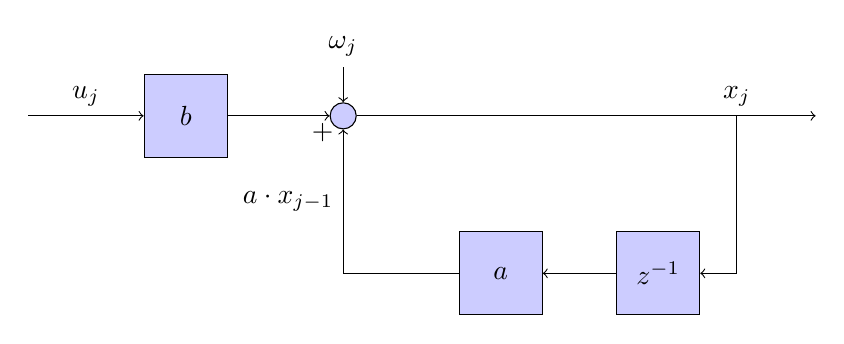
\begin{tikzpicture}[auto, node distance=2cm]
 
	% Input
	\node [input, name=input] {};
 
	% b gain
	\node [block, right of=input] (b) {$b$};
 
	% sum element
	\node [sum, right of=b,
			pin={[pinstyle]above:$\omega_j$},
         	node distance=2cm] (sum) {};
 
	% Two silent nodes in the middle 
	\node [output, right of=sum] (x1) {};
	\node [output, right of=x1] (x2) {};
 
	% Output node
	\node [output, right of=x2] (output) {};
 
	% Nodes in the feedback loop
	\node [block, below of=x2] (delay) {$z^{-1}$};
	\node [block, below of=x1] (a) {$a$};
	
	% Once the nodes are placed, connecting them is easy. 
	\draw [draw,->] (input) -- node {$u_j$} (b);
	\draw [->] (b) -- (sum);
	\draw [-] (sum) -- (x1);
	\draw [-] (x1) -- (x2);
	\draw [->] (x2) -- node [name=y] {$x_j$}(output);
	\draw [->] (y) |- (delay);
	\draw [->] (delay) -- (a);
	\draw [->] (a) -| node[pos=0.99] {$+$} 
     		node [near end] {$a \cdot x_{j-1}$} (sum);
\end{tikzpicture}

\caption{text}
\end{figure}

Almost always random phenomena are hidden from the observer behind a dynamical system - Kalman described this as follows:\\

\textit{A random function of time may be thought of as the output of a dynamic system excited by an independent Gaussian random process.} \cite{Kalman:1960}\\

This is true for robotic motion, given that we can only attempt to estimate the robot's stochastically perturbed motion, through the use of sensors like odometry, or laser range finders, which are subject to stochastic noise. Letting the measurement of signal $x_j$ be represented by $z_j$, we can write the following equation defining the measurement of $x_j$ as:
\begin{equation}
z_j = h \cdot x_j + \nu_j
\end{equation} 

Equation (2) can be represented in a computational graph as follows:
\begin{figure}[h]
\centering
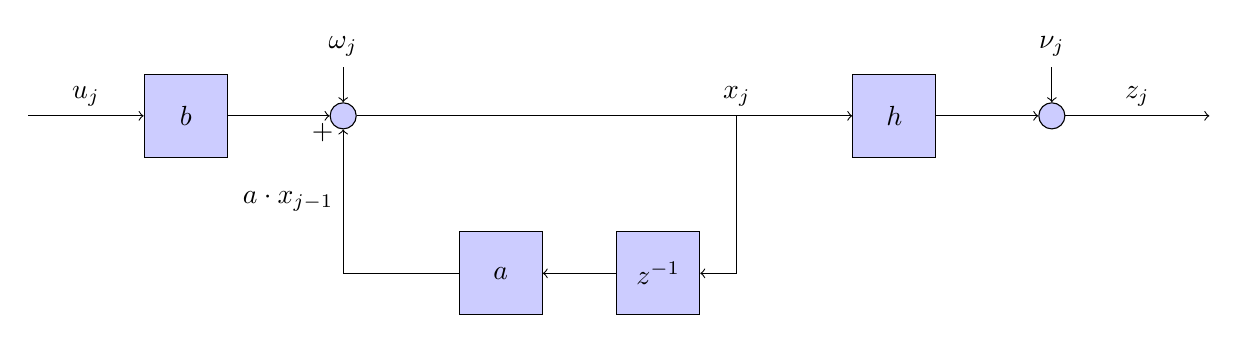
\begin{tikzpicture}[auto, node distance=2cm]

    % Input
    \node [input, name=input] {};
    
    % b gain
    \node [block, right of=input] (b) {$b$};
    
    % sum element
    \node [sum, right of=b,
    pin={[pinstyle]above:$\omega_j$},
            node distance=2cm] (sum) {};
    
    % Two silent nodes in the middle
    \node [output, right of=sum] (x1) {};
    \node [output, right of=x1] (x2) {};
	 
	% Output node
    \node [output, right of=x2] (output) {};
    
    % Nodes in the feedback loop
    \node [block, below of=x2] (delay) {$z^{-1}$};
	\node [block, below of=x1] (a) {$a$};
	
	% Gain on the xj signal
	\node [block, right of=output, node distance=1cm] (h) {$h$};
	
	% sum node
	\node [sum, right of=h,
	    pin={[pinstyle]above:$\nu_j$},
	            node distance=2cm] (sum2) {};
	            
	% measurement output
	\node [output, right of=sum2] (output2) {};
	
    % Once the nodes are placed, connecting them is easy. 
    \draw [draw,->] (input) -- node {$u_j$} (b);
    \draw [->] (b) -- (sum);
    \draw [-] (sum) -- (x1);
    \draw [-] (x1) -- (x2);
    \draw [-] (x2) -- node [name=y] {$x_j$}(output);
    \draw [->] (y) |- (delay);
    \draw [->] (delay) -- (a);
    \draw [->] (a) -| node[pos=0.99] {$+$} 
        node [near end] {$a \cdot x_{j-1}$} (sum);
    
    % measurement section
    \draw [->] (output) -- (h);
    \draw [->] (h) -- (sum2);
    \draw [->] (sum2) -- node [name=y2] {$z_j$}(output2);
\end{tikzpicture}
\caption{text}
\end{figure}

The fundamental problem that the Kalman Filter tries to answer is: how can an accurate estimate of a hidden stochastic signal be found when it is observed as the output of a dynamical system? The first step to answering this is to create a mathematical model of the system we can use to find an estimate of the measurement, $z_j$, which we call $\hat{z_j}$. This estimate is based on an estimation of the hidden variable, which we denote with $\hat{x_j}$. The mathematical model that provides these estimates does not factor in stochasticity seen in actual signals $x_j$ and $z_j$. The estimation architecture can be seen in Figure 3.
\begin{figure}[h]
\centering
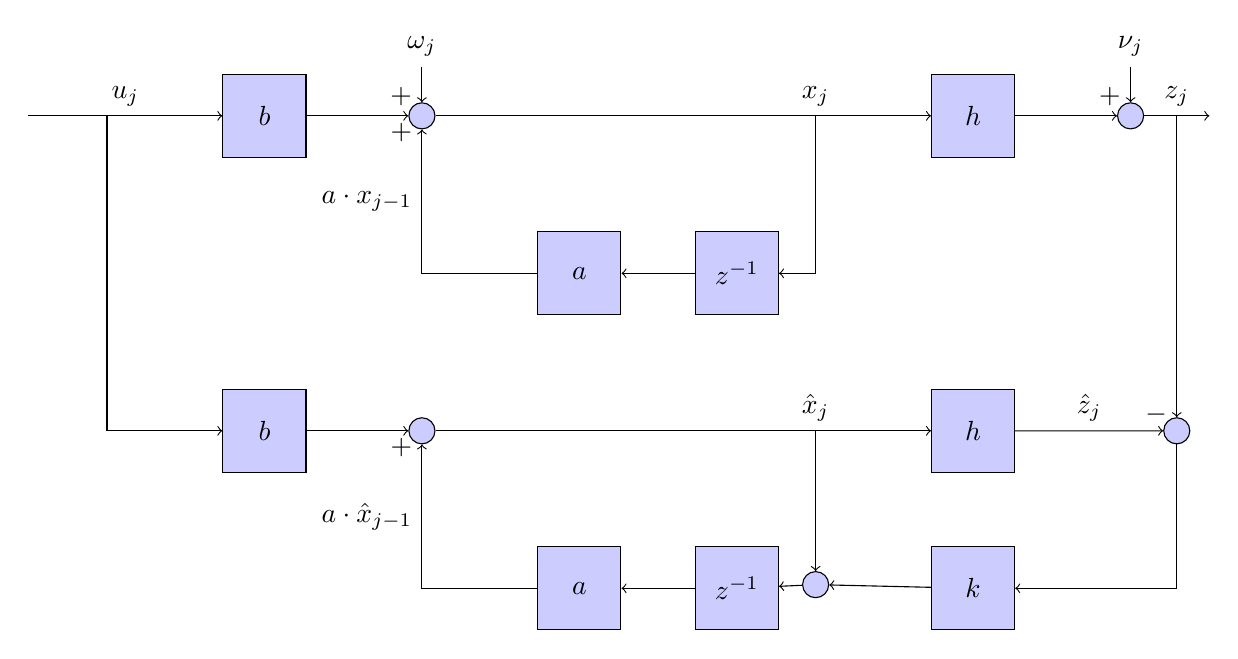
\begin{tikzpicture}[auto, node distance=2cm]
	% % % % % % % % % % % % % % % % % % % % % % %
    % Upper model
    % % % % % % % % % % % % % % % % % % % % % % %
    % Input
    \node [input, name=input] {};
    \node [input, left of=input, node distance=1cm] (start) {};
    
    % b gain
    \node [block, right of=input] (b) {$b$};
    
    % sum element
    \node [sum, right of=b,
    pin={[pinstyle]above:$\omega_j$},
            node distance=2cm] (sum) {};
    
    % Two silent nodes in the middle
    \node [output, right of=sum] (x1) {};
    \node [output, right of=x1] (x2) {};
	 
	% Output node
    \node [output, right of=x2] (output) {};
    
    % Nodes in the feedback loop
    \node [block, below of=x2] (delay) {$z^{-1}$};
	\node [block, below of=x1] (a) {$a$};
	
	% Gain on the xj signal
	\node [block, right of=output, node distance=1cm] (h) {$h$};
	
	% sum node
	\node [sum, right of=h,
	    pin={[pinstyle]above:$\nu_j$},
	            node distance=2cm] (sum2) {};
	            
	% measurement output
	\node [output, right of=sum2, node distance=1cm] (output2) {};
	
    % Once the nodes are placed, connecting them is easy. 
    %\draw [draw,->] (start) -- (input);
    \draw [draw,->] (start) -- node {$u_j$} (b);
    \draw [->] (b) -- node[pos=0.93] {$+$} (sum);
    \draw [-] (sum) -- (x1);
    \draw [-] (x1) -- (x2);
    \draw [-] (x2) -- node [name=y] {$x_j$}(output);
    \draw [->] (y) |- (delay);
    \draw [->] (delay) -- (a);
    \draw [->] (a) -| node[pos=0.99] {$+$} 
        node [near end] {$a \cdot x_{j-1}$} (sum);
    
    % measurement section
    \draw [->] (output) -- (h);
    \draw [->] (h) -- node[pos=0.93] {$+$} (sum2);
    \draw [->] (sum2) -- node [name=y2] {$z_j$}(output2);
    
    
    % % % % % % % % % % % % % % % % % % % % % % %
    % Lower model
    % % % % % % % % % % % % % % % % % % % % % % %
    
    % lower b node
    \node [block, below of=b, node distance=4cm] (be) {$b$};
    
    % sum element
    \node [sum, right of=be, node distance=2cm] (sume) {};
        
    % Two silent nodes in the middle
    \node [output, right of=sume] (x1e) {};
    \node [output, right of=x1e] (x2e) {};
    	 
    % Output node
    \node [output, right of=x2e] (outpute) {};
        
    % Nodes in the feedback loop
    \node [block, below of=x2e] (delaye) {$z^{-1}$};
    \node [block, below of=x1e] (ae) {$a$};
    
    % Gain on the xj signal
    \node [block, right of=outpute, node distance=1cm] (he) {$h$};
    		            
    % measurement output
    \node [output, right of=he] (output2e) {};
    
    \node [sum, below of=y2, node distance=4.25cm] (sum2e) {};
    
    \node [block, below of=he] (k) {$k$};
    
    % Once the nodes are placed, connecting them is easy.
    \draw [->] (input) |- (be);
    \draw [->] (be) -- (sume);
    \draw [-] (sume) -- (x1e);
    \draw [-] (x1e) -- (x2e);
    \draw [-] (x2e) -- node [name=ye] {$\hat{x}_j$}(outpute);
    %\draw [->] (ye) |- (delaye);
    \draw [->] (delaye) -- (ae);
    \draw [->] (ae) -| node[pos=0.99] {$+$} 
            node [near end] {$a \cdot \hat{x}_{j-1}$} (sume);
        
    % measurement section
    \draw [->] (outpute) -- (he);
    \draw [->] (he) -- node [name=y2e] {$\hat{z}_j$}(sum2e);
    
    \draw [->] (y2) -- node[left, pos=0.99] {$-$} (sum2e);
    
    \node [sum, below of=ye, node distance=2.25cm] (sumfin) {};
    
    \draw [->] (sum2e) |- (k);
    \draw [->] (ye) -- (sumfin);
    \draw [->] (k) -- (sumfin);
    \draw [->] (sumfin) -- (delaye);
    
\end{tikzpicture}
\caption{text}
\end{figure}

\subsection{Particle Filters}
Particle filters can be used to solve the global localisation problem, that is, it can localise a robot in an environment when its initial position is unknown. This section looks at a specific type of particle filter known as Monte Carlo Localisation (MCL). The central idea of MCL is the posterior distribution estimation of the robot poses, often referred to as the \textit{belief}. The \textit{belief} is defined as probability density over the pose state space, which is conditioned on sensor measurement data, and odometric action data. Mobile robot pose, $\mathbf{x}$, is made up of location coordinates $x$ and $y$ and orientation $\theta$. Letting observation from a laser range finder be represented by $\mathbf{o}$, and odometric sensor data by represented by $\mathbf{a}$, we can mathematically express the belief as follows:
\begin{equation}
Bel(\mathbf{x}_t) = p(\mathbf{x}_t | \mathbf{o}_t, \mathbf{a}_{t-1}, \mathbf{o}_{t-1}, \mathbf{a}_{t-2},\ldots,\mathbf{o}_0)
\end{equation}

Particle filters estimate belief recursively, meaning that an update rule from time $t$ to time $t+1$ is required, and an initial belief is also needed. The initial belief characterizes the initial knowledge about the system state - if little is known about the initial system state, then a uniform distribution can be used over the state space. To derive the update equation we start by expressing (3) using Bayes rule:
\begin{equation}
Bel(\mathbf{x}_t) = \frac{p(\mathbf{o}_t | \mathbf{x}_t,\mathbf{a}_{t-1},\ldots,\mathbf{o}_0) \ p(\mathbf{x}_t | \mathbf{a}_{t-1},\ldots,\mathbf{o}_0)}{p(\mathbf{o}_t | \mathbf{a}_{t-1},\ldots,\mathbf{o}_0)}
\end{equation}

The denominator is a constant value relative to $\mathbf{x}_t$, and (4) can be written more compactly as:
\begin{equation}
Bel(\mathbf{x}_t) = \eta \ p(\mathbf{o}_t | \mathbf{x}_t,\mathbf{a}_{t-1},\ldots,\mathbf{o}_0) \ p(\mathbf{x}_t | \mathbf{a}_{t-1},\ldots,\mathbf{o}_0)
\end{equation}

where $\eta$ is a constant value:
\begin{equation}
\eta = p(\mathbf{o}_t | \mathbf{a}_{t-1},\ldots,\mathbf{o}_0)^{-1}
\end{equation}

A recursive relation seeks to provide an update at each time step. Information from the past is factored into the belief as changes occur. Therefore it can be reasoned that only new information presented to the system from current state is important when modifying the belief. This simplifying assumption, referred to as the \textit{Markov assumption}, suggests that future data is independent of past data given knowledge of the current state. Mathematically, this allows equation (5) to be re-written as:
\begin{equation}
Bel(\mathbf{x}_t) = \eta \ p(\mathbf{o}_t | \mathbf{x}_t) \ p(\mathbf{x}_t | \mathbf{a}_{t-1},\ldots,\mathbf{o}_0)
\end{equation} 

Partitioning over $\mathbf{x}_{t-1}$ equation (7) can be written as:
\begin{equation}
Bel(\mathbf{x}_t) = \eta \ p(\mathbf{o}_t | \mathbf{x}_t) \int p(\mathbf{x}_t, \mathbf{x}_{t-1} | \mathbf{a}_{t-1},\ldots,\mathbf{o}_0) \ d\mathbf{x}_{t-1}
\end{equation}

Applying Bayes' equation (8) can be written as:
\begin{equation}
Bel(\mathbf{x}_t) = \eta \ p(\mathbf{o}_t | \mathbf{x}_t) \int p(\mathbf{x}_{t} | \mathbf{x}_{t-1},\mathbf{a}_{t-1},\ldots,\mathbf{o}_0) \ p(\mathbf{x}_{t-1} | \mathbf{a}_{t-1},\ldots,\mathbf{o}_0) \ d\mathbf{x}_{t-1}
\end{equation}

Exploiting the Markov property again the first expression in the integral can be simplified. The second expression can be written using the $Bel$ notation as follows:
\begin{equation}
Bel(\mathbf{x}_t) = \eta \ p(\mathbf{o}_t | \mathbf{x}_t) \int p(\mathbf{x}_{t} | \mathbf{x}_{t-1},\mathbf{a}_{t-1}) \ Bel(\mathbf{x}_{t-1}) \ d\mathbf{x}_{t-1}
\end{equation}

\subsection{Comparison \& Model Selection}
Compare the two approaches and determine which approach was implemented to provide localisation for the two robot models.

\section{Simulations}
Describe the performance of the robots. Show the two robot model designs, highlighting the placement of sensors, and the sensors that were employed for the robot.

\subsection{Achievements}

\subsection{Benchmark Model}
\subsubsection{Model Design}
the size of the robot, the layout of the sensors - use a chart or a table

\subsubsection{Packages Used}


\subsubsection{Parameters}

\subsection{Personal Model}

\section{Results}
\subsection{Localisation}
\subsection{Technical Comparison}

\section{Discussion}

\subsection{Topics}

\section{Conculsion / Future Work}
\subsection{Modifications for Improvement}
\subsection{Hardward Deployment}

\bibliography{my_bib}
\bibliographystyle{ieeetr}

\end{document}